\documentclass[main]{subfiles}
\begin{document}
%@@@@@@@@@@@@@@@@@@@@@@@@@@@@@@
% summarizes lecture 6
% author: Doris Ling

\section{Current Conveyor}
% Doris
The Current Conveyor, also commonly known as a Buffered Current Mirror, consists of two transistors. where the $M_1$ gate is tied to the $M_2$ drain, and the $M_2$ gate is tied to the $M_1$ source as shown in Figure \ref{fig:Current_Conveyor_circuit}.

\begin{figure}[htbp]
  \centering
  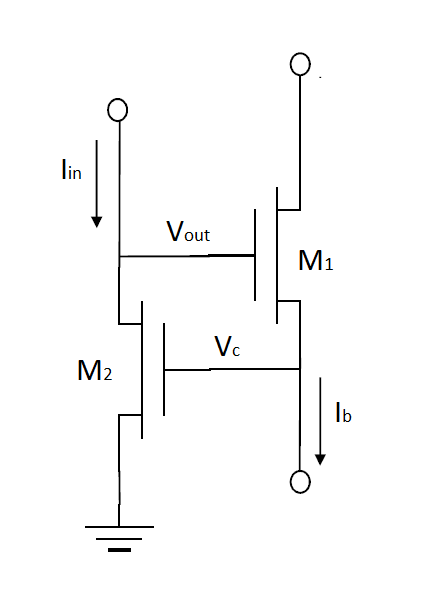
\includegraphics[scale=0.5]{pics/Current_Conveyor_circuit.png}
  \caption{Current Conveyor circuit}
  \label{fig:Current_Conveyor_circuit}
\end{figure}
The Current Conveyor acts like a source follower ($M_1$) whose output terminal is tied to the gate of a current sink ($M_2$). The input current, $I_{in}$, will charge $V_{out}$ to turn on $M_1$ whose current will charge $V_c$, turning on $M_2$ until $M_2$ sinks $I_{in}$. The current being sunk by $M_2$ follows $V_c$ according to:

\begin{equation}
I =  e^{\kappa*V_c} \geq 0
\end{equation}  
\end{document}